\documentclass[aspectratio=169]{beamer}

\usetheme{default}

\usepackage[utf8]{inputenc}
\usepackage[russian]{babel}
\usepackage[OT1]{fontenc}
\usepackage{amsmath}
\usepackage{amsfonts}
\usepackage{amssymb}
\usepackage{graphicx}
\usepackage{etoolbox}
\usepackage{caption}
\usepackage{subcaption}
\captionsetup{compatibility=false}
\usepackage{pifont}
%\usepackage{subfigure}
\usepackage{xcolor}
\usepackage{framed}
\usepackage{empheq}
\usepackage[many]{tcolorbox}
\usepackage{multirow}
\usepackage{tikz}
\usepackage{listings}
\usepackage{tikz}

\definecolor{shadecolor}{cmyk}{0,0,0,1}

\lstset{
	backgroundcolor=\color{lightgray},
	commentstyle=\color{blue},
	frame=single
	breakatwhitespace, 
	language=python, 
	columns=fullflexible, 
	keepspaces, 
	breaklines, 
	tabsize=3, 
	showstringspaces=false, 
	extendedchars=true,
	numbers=left
}

\makeatletter

\setbeamercolor{title}{fg=white}
\setbeamercolor{frametitle}{fg=black}
\setbeamerfont*{title}{family=\sffamily,size=\LARGE}

\setbeamerfont{page number in head/foot}{size=\scriptsize}
\setbeamertemplate{footline}[frame number]
\let\otp\titlepage
\renewcommand{\titlepage}{\otp\addtocounter{framenumber}{-1}}

\setbeamertemplate{background canvas}{%
	\ifnumequal{\c@framenumber}{0}{%
		\vbox to \paperheight{\vfil\hbox to \paperwidth{\hfil
\includegraphics[height=\paperheight]{images/cover.png}\hfil}\vfil}
   }{%
      \ifnumequal{\c@framenumber}{\inserttotalframenumber}{
        \vbox to \paperheight{\vfil\hbox to \paperwidth{\hfil
\includegraphics[height=\paperheight]{images/back.png}\hfil}\vfil}
      }{%
         % Other frames
      }%
   }%
}

\makeatother

\beamertemplatenavigationsymbolsempty

\tcbset{highlight math style={enhanced,colframe=red,colback=white,arc=4pt,boxrule=1pt}}

\usetikzlibrary{shadings,shadows,shapes.arrows}

\newcommand*{\tikzarrow}[2]{%
  \tikz[
    baseline=(A.base),             % Set baseline to the baseline of node content
    font=\footnotesize\sffamily    % Set fontsize of the node content
  ]
  \node[
    single arrow,                  % Shape of the node
    single arrow head extend=5pt,  % Actual width of arrow head
    draw,                          % Draw the node shape
    inner sep=3pt,                 % Separation between node content and node shape
    top color=#1,               % Shading color on top of node
    bottom color=#1,               % Shading color on bottom of node
    % drop shadow                    % Draw a shadow
  ] (A) {#2};%
}

\newcommand{\tikzfancyarrow}[2][2cm]{\tikz[baseline=-0.5ex]\node [arrowstyle=#1] {#2};}
\newcommand*\rot{\rotatebox{90}}

\author{Николай Анохин}
\title{\newline \newline \newline Лекция 6 \\ Деревья принятия решений}

\begin{document}

\begin{frame}[plain]
\titlepage
\end{frame}

\begin{frame}{План занятия}
\tableofcontents
\end{frame}

% ========================================
\section{Деревья решений}
% ========================================

\begin{frame}{}

\begin{center}
\Large Деревья решений
\end{center}

\end{frame}

\begin{frame}{Задача}

\begin{columns}[T]
    \begin{column}{.5\textwidth}
    {\bf Дано:}
    
		обучающая выборка из профилей нескольких десятков тысяч человек
		\begin{itemize}
		\item пол (binary)
		\item возраст (numeric)
		\item образование (nominal)
		\item и еще 137 признаков
		\item наличие интереса к косметике
		\end{itemize} 

	{\bf Задача:}

	Для рекламной кампании определить, характеристики людей, интересующихся косметикой
     
    \end{column}
    \begin{column}{.5\textwidth}
    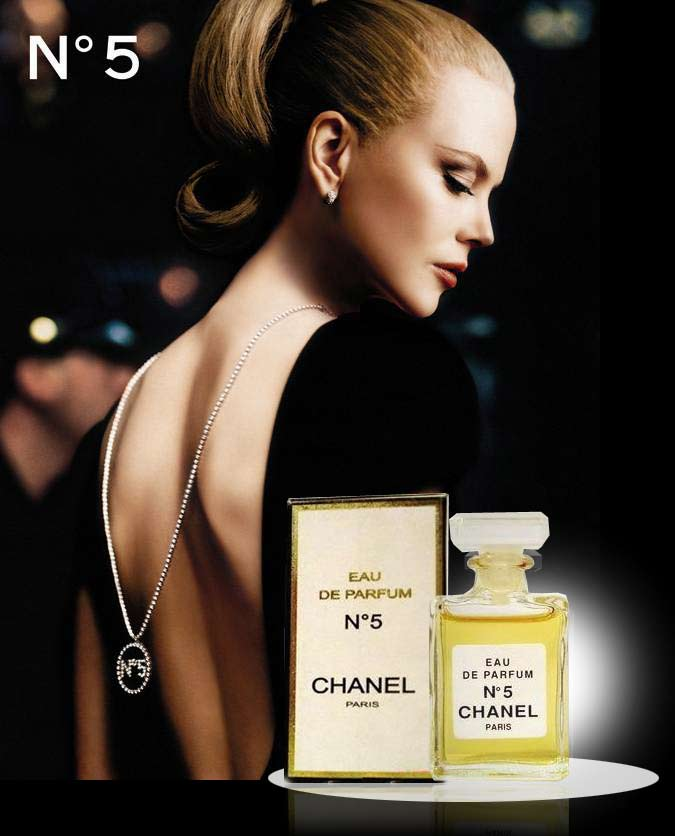
\includegraphics[scale=0.23]{images/nicole.jpg}    
    \end{column}
  \end{columns}
  
\end{frame}

\begin{frame}{Обама или Клинтон?}

\begin{center}
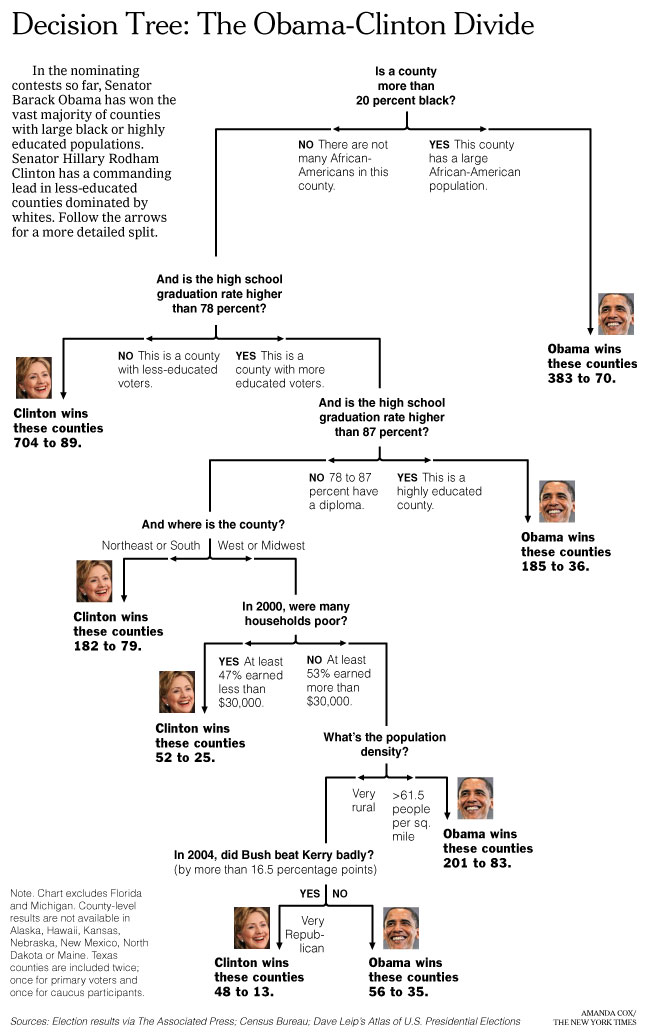
\includegraphics[scale=0.33]{images/obama.jpg}
\end{center}

\end{frame}

\begin{frame}{Хороший день для партии в гольф}

\begin{center}
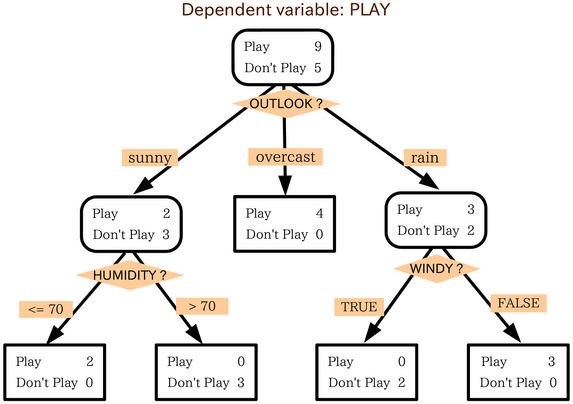
\includegraphics[scale=0.33]{images/golf.png}
\end{center}

\end{frame}

\begin{frame}{Регионы принятия решений}

\begin{center}
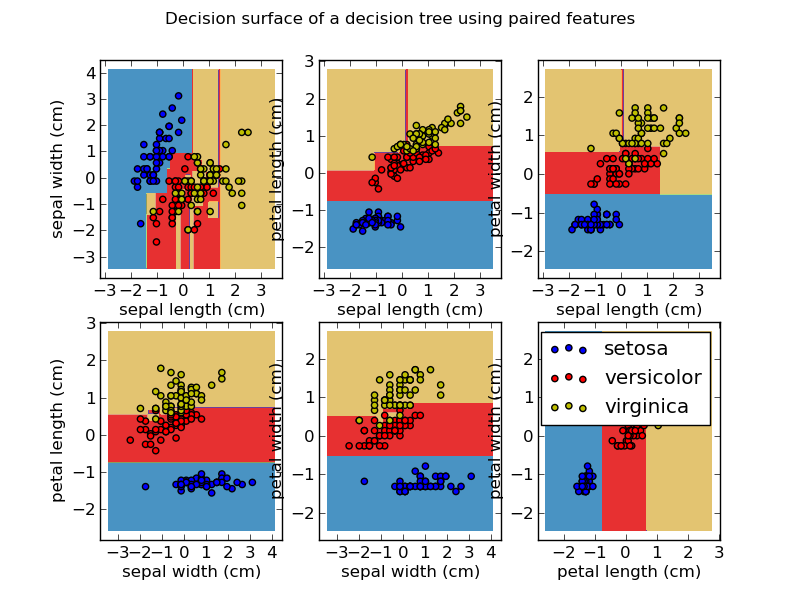
\includegraphics[scale=0.45]{images/regions.png}
\end{center}

\end{frame}

\defverbatim[colored]\dt{%
\begin{lstlisting}[tabsize=4,basicstyle=\ttfamily]
function decision_tree(X_N):
	if X_N satisfies leaf criterion:
		L = create_leaf(X_N)
		assign_class(L)
	else:
		L = create_node(X_N)
		X_1,..,X_S = split(L)
		for i in 1..S:
			C = decision_tree(X_i)
			add_child(L, C)
	return L
\end{lstlisting}
}

\begin{frame}{Рекурсивный алгоритм}

\dt

\end{frame}

\begin{frame}{CART}

Classification And Regression Trees

\begin{enumerate}
\item Как происходит разделение?
\item На сколько детей разделять каждый узел?
\item Какой критерий листа выбрать?
\item Как укоротить слишком большое дерево?
\item Как выбрать класс каждого листа?
\item Что делать, если часть значений отсутствует?
\end{enumerate}

\end{frame}

\begin{frame}{Чистота узла}

\begin{block}{Задача}
Выбрать метод, позволяющий разделить узел на два или несколько детей наилучшим образом
\end{block}

\vspace{1em}
Ключевое понятие -- {\it impurity} узла.
\begin{enumerate}
\item Misclassification
\[
i(N) = 1 - \max_k p(x \in C_k)
\]
\item Gini
\[
i(N) = 1 - \sum_k p^2(x \in C_k) = \sum_{i \neq j} p(x \in C_i) p(x \in C_j)
\]
\item Информационная энтропия
\[
i(N) =  -\sum_k p(x \in C_k) \log_2 p(x \in C_k)
\]
\end{enumerate}

\end{frame}

\begin{frame}{Теория информации}

Количество информации $\thicksim$ ``степень удивления''
\[
h(x) = -\log_2 p(x)
\]
Информационная энтропия $H[x] = E[h(x)]$
\[
H[x] = -\sum p(x) \log_2 p(x) \;\;\text{или}\;\; H[x] = - \int p(x) \log_2 p(x) dx
\]
\begin{exampleblock}{Упражнение}
Дана случайная величина $x$, принимающая 4 значения с равными вероятностями $\frac 1 4$, и случайная величина $y$, принимающая 4 значения с вероятностями $\{\frac 1 2, \; \frac 1 4, \; \frac 1 8, \; \frac 1 8\}$. Вычислить $H[x]$ и $H[y]$.
\end{exampleblock}

\end{frame}

\begin{frame}{Выбор наилучшего разделения}

\begin{block}{Критерий}
Выбрать признак и точку отсечения такими, чтобы было максимально уменьшение $impurity$
\[
\Delta i(N, N_L, N_R) = i(N) - \frac {N_L}{N} i(N_L) - \frac {N_R}{N} i(N_R)
\]
\end{block}

\vspace{1em}
Замечания
\begin{itemize}
\item Выбор границы при числовых признаках: середина?
\item Решения принимаются локально: нет гарантии глобально оптимального решения
\item На практике выбор impurity не сильно влияет на результат
\end{itemize}

\end{frame}

\begin{frame}{Если разделение не бинарное}

Естественный выбор при разделении на $B$ детей
\[
\Delta i(N, N_1, \ldots, N_B) = i(N) - \sum_{k=1}^B \frac{N_k}{N} i(N_k) \rightarrow \max
\]
Предпочтение отдается большим $B$. Модификация:
\[
\Delta i_B(N, N_1, \ldots, N_B) = \frac{\Delta i(N, N_1, \ldots, N_B)}{-\sum_{k=1}^B \frac{N_k}{N} \log_2 \frac{N_k}{N}} \rightarrow \max
\]
(gain ratio impurity)

\end{frame}

\begin{frame}{Использование нескольких признаков}

\begin{center}
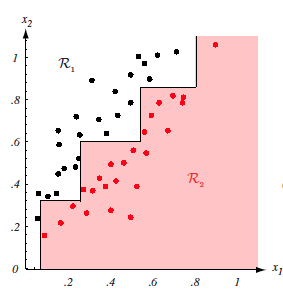
\includegraphics[scale=0.45]{images/multi1.png}\;
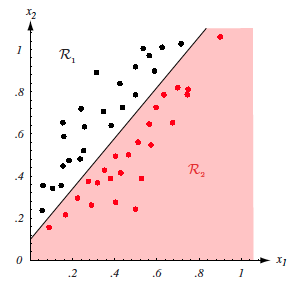
\includegraphics[scale=0.45]{images/multi2.png}
\end{center}

\end{frame}

\begin{frame}{Практика}

\begin{exampleblock}{Задача}
Вычислить наилучшее бинарное разделение корневого узла по одному признаку, пользуясь gini impurity.

\begin{center}
\begin{tabular}{| l | c | c | c | c |}
\hline
\textnumero & {\bf Пол} & {\bf Образование} & {\bf Работа} & {\bf Косметика} \\
\hline
1 & М & Высшее & Да & Нет \\
2 & М & Среднее & Нет & Нет \\
3 & М & Нет & Да & Нет \\
4 & М & Высшее & Нет & Да \\
1 & Ж & Нет & Нет & Да \\
2 & Ж & Высшее & Да & Да \\
3 & Ж & Среднее & Да & Нет \\
4 & Ж & Среднее & Нет & Да \\
\hline
\end{tabular}
\end{center}
\end{exampleblock}

\end{frame}

\begin{frame}{Когда остановить разделение}

Split stopping criteria
\begin{itemize}
\item никогда
\item использовать валидационную выборку
\item установить минимальный размер узла
\item установить порог $\Delta i(N) > \beta$
\item статистический подход
\[
\chi^2 = \sum_{k=1}^2 \frac{(n_{kL} - \frac{N_L}{N} n_{k})^2}{\frac{N_L}{N} n_{k}}
\]
\end{itemize}

\end{frame}

\begin{frame}{Укорачиваем дерево}

Pruning (a.k.a. отрезание ветвей)
\begin{enumerate}
\item Растим ``полное'' дерево $T_0$
\item На каждом шаге заменяем самый ``слабый'' внутренний узел на лист
\[
R_{\alpha}(T_k) = err(T_k) + \alpha size(T_k)
\]
\item Для заданного $\alpha $ из получившейся последовательности 
\[
T_0 \succ T_1 \succ \ldots \succ T_r
\]
выбираем дерево $T_k$, минимизирующее $R_{\alpha}(T_k)$
\end{enumerate}
Значение $\alpha$  выбирается на основании тестовой выборки или CV

\end{frame}

\begin{frame}{Какой класс присвоить листьям}

\begin{enumerate}
\item Простейший случай: \\ класс с максимальным количеством объектов
\item Дискриминативный случай: \\ вероятность $p(C_k | x)$
\end{enumerate}

\end{frame}

\begin{frame}{Вычислительная сложность}

Выборка состоит из $n$ объектов, описанных $m$ признаками

\vspace{1em}
Предположения
\begin{enumerate}
\item Узлы делятся примерно поровну
\item Дерево имеет $\log n$ уровней
\item Признаки бинарные
\end{enumerate}

\vspace{1em}
{\bf Обучение. } Для узла с $k$ обучающими объектами:

\vspace{1em}
\hspace{1em}Вычисление impurity по одному признаку $O(k)$

\hspace{1em}Выбор разделяющего признака $O(mk)$ 

\hspace{1em}Итог: $O(mn) + 2 O(m \frac{n}{2}) + 4 O(m \frac{n}{4}) + \ldots = O(m n \log n)$

\vspace{1em}
{\bf Применение. } $O(\log n)$

\end{frame}

\begin{frame}{Отсутствующие значения}

\begin{itemize}
\item Удалить объекты из выборки
\item Использовать отстутсвие как отдельную категорию
\item Вычислять impurity, пропуская отсутствующие значения
\item Surrogate splits: разделяем вторым признаком так, чтобы было максимально похоже на первичное разделение
\end{itemize}

\end{frame}

\begin{frame}{Surrogate split}
\vspace{-1em}
\[
c_1: \quad 
x_1=\begin{pmatrix}0 \\ 7 \\ 8\end{pmatrix},\;
x_2=\begin{pmatrix}1 \\ 8 \\ 9\end{pmatrix},\;
x_3=\begin{pmatrix}2 \\ 9 \\ 0\end{pmatrix},\;
x_4=\begin{pmatrix}4 \\ 1 \\ 1\end{pmatrix},\;
x_5=\begin{pmatrix}5 \\ 2 \\ 2\end{pmatrix}
\]
\[
c_2: \quad 
y_1=\begin{pmatrix}3 \\ 3 \\ 3\end{pmatrix},\;
y_2=\begin{pmatrix}6 \\ 0 \\ 4\end{pmatrix},\;
y_3=\begin{pmatrix}7 \\ 4 \\ 5\end{pmatrix},\;
y_4=\begin{pmatrix}8 \\ 5 \\ 6\end{pmatrix},\;
y_5=\begin{pmatrix}9 \\ 6 \\ 7\end{pmatrix}
\]
\begin{center}
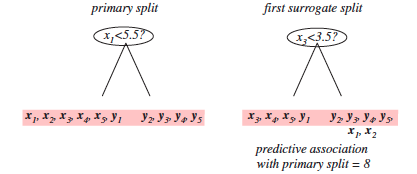
\includegraphics[scale=0.5]{images/surrogate2.png}
\end{center}

\begin{exampleblock}{Упражнение}
Вычислить второй surrogate split
\end{exampleblock}

\end{frame}

\begin{frame}{Задача о косметике}

\begin{center}
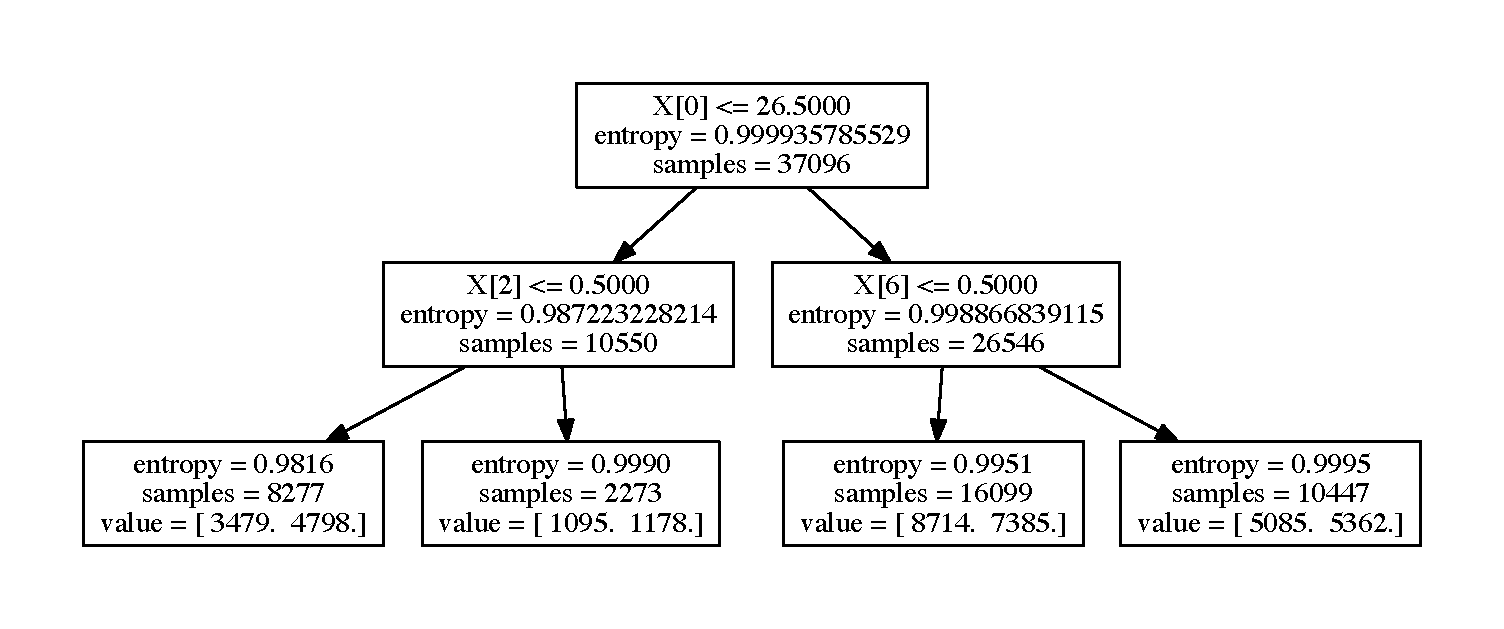
\includegraphics[scale=0.45]{images/model.pdf}
\end{center}

$X_0$ -- возраст, $X_2$ -- неоконченное высшее образование, $X_6$ - пол

\end{frame}

\begin{frame}{Задачи регрессии}

Impurity узла N
\[
i(N) = \sum_{y \in N} (y - \overline{y})^2
\]

Присвоение класса листьям
\begin{itemize}
\item Среднее значение
\item Линейная модель
\end{itemize}

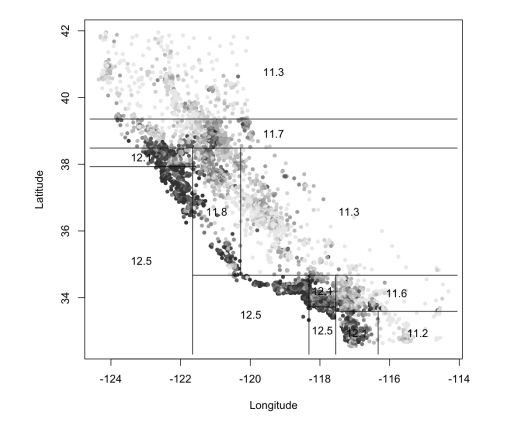
\includegraphics[scale=0.3]{images/housing.png}

\end{frame}

\begin{frame}{Кроме  CART}

\begin{itemize}

\item[ID3] Iterative Dichotomiser 3 
	\begin{itemize}
	\item Только номинальные признаки
	\item Количество детей в узле $=$ количество значений разделяющего признака
	\item Дерево растет до максимальной высоты
	\end{itemize}
	
\item[С4.5] Улучшение ID3
	\begin{itemize}
	\item Числовые признаки -- как в CART, номинальные -- как в ID3
	\item При отсутствии значения используются {\bf все} дети
	\item Укорачивает дерево, убирая ненужные предикаты в правилах
	\end{itemize}
	
\item[C5.0] Улучшение C4.5
	\begin{itemize}
	\item Проприетарный
	\end{itemize}
		
\end{itemize}

\end{frame}

\begin{frame}{Решающие деревья. Итог}

\begin{itemize}
\item[+] Легко интерпретируемы. Визуализация (ня!)
\item[+] Любые входные данные
\item[+] Мультикласс из коробки
\item[+] Предсказание за $O(\log n)$
\item[+] Поддаются статистическому анализу
\end{itemize}

\begin{itemize}
\item[--] Склонны к переобучению
\item[--] Жадные и  нестабильные
\item[--] Плохо работают при дисбалансе классов
\end{itemize}

\end{frame}

\begin{frame}{Ключевые фигуры}

\begin{columns}[T]
    \begin{column}{.5\textwidth}
    	\vspace{5em}
    	\begin{itemize}
			\item Claude Elwood Shannon \\ (Теория информации)
			\item Leo Breiman \\ (CART, RF)
			\item John Ross Quinlan  \\ (ID3, C4.5, C5.0)
		\end{itemize}        
    \end{column}
    \begin{column}{.5\textwidth}
    \begin{center}
    	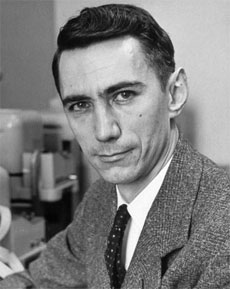
\includegraphics[scale=0.3]{images/shannon.jpg}\, 	   
	   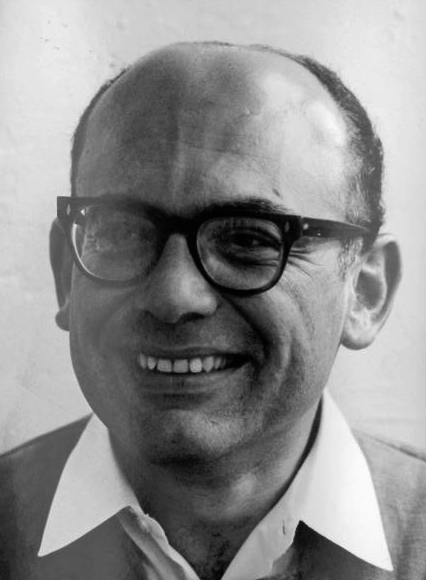
\includegraphics[scale=0.3115]{images/breiman.png}
	   	   
	   \vspace{0.3em}
	   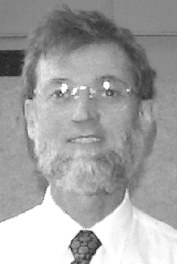
\includegraphics[scale=0.32]{images/quinlan.png} 
    \end{center}	   
    \end{column}
  \end{columns}

\end{frame}

\begin{frame}[plain]
\begin{center}
{\Large Вопросы}
\end{center}
\end{frame}

\end{document}